% Fichier généré automatiquement par tools/generate_corrections.py.
% Source : DYN/DYN-04-TorseurDynamique/STOCK/14_Sympact/14_Sympact.tex
% Statut : complété (3/3 question(s)).
\begin{corrigebox}[Corrigé complété]
\CorrigeQuestion{1}
On construit un sommet par solide, puis une arête par liaison en
        indiquant son type, son centre et son axe. Les actions extérieures (poids,
        actionneur, charge) sont reliées au solide concerné. Le graphe doit retrouver le
        nombre de mobilités et de boucles du mécanisme de l'énoncé.
\CorrigeQuestion{2}
\CorrigeSource{Réponse reprise d'un exercice homonyme de la banque ; la provenance exacte est indiquée dans le commentaire du fichier.}
% Réponse reprise de : GEO/GEO-01/14_Sympact/14_Sympact.tex
\begin{center}
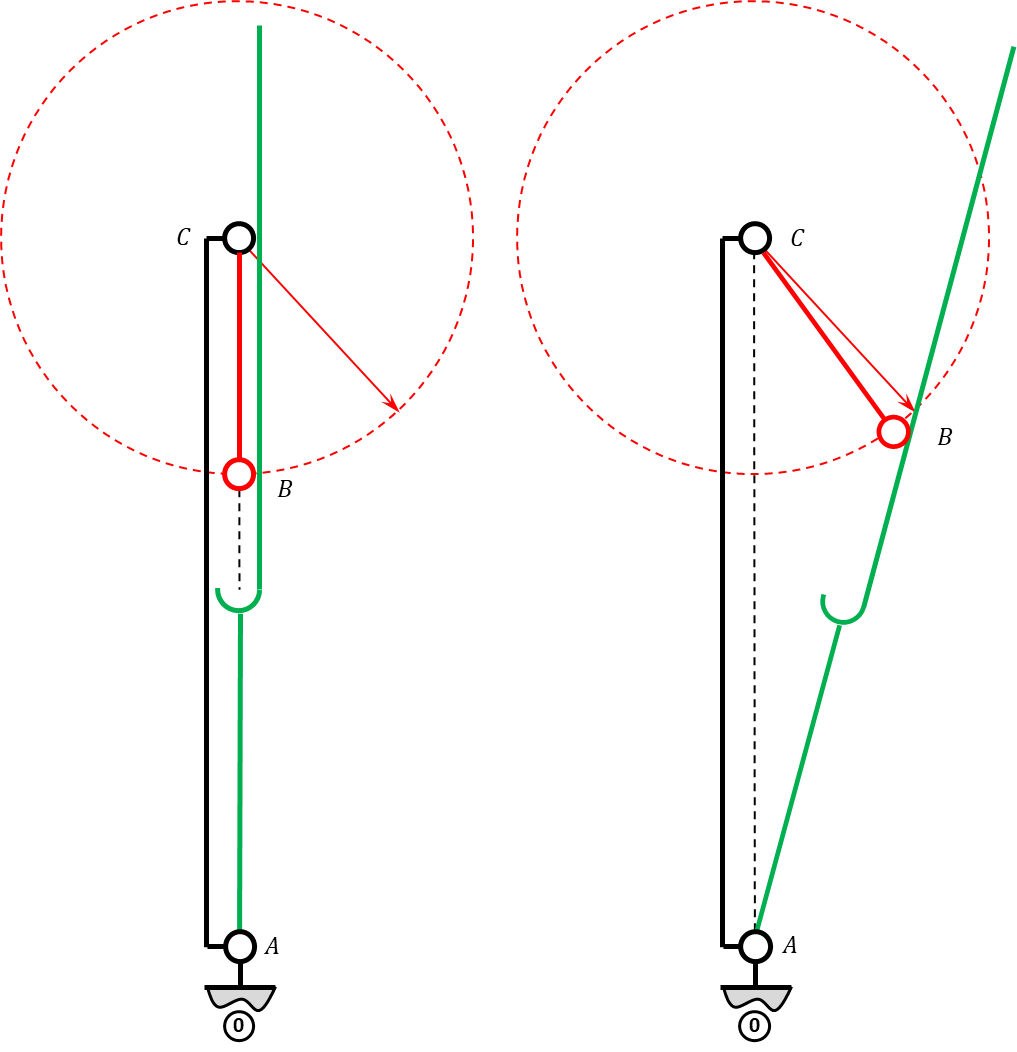
\includegraphics[width=.5\linewidth]{../../../../../02-Modélisation des mécanismes/TD/Géométrie/14_Sympact/images/14_01_c}
\end{center}
\CorrigeQuestion{3}
Le schéma est reconstruit en conservant uniquement les axes, centres,
        directions de glissière et longueurs fonctionnelles. Les angles et courses imposés
        sont appliqués dans l'ordre de la chaîne cinématique; les liaisons doivent rester
        fermées et les contacts sans pénétration.
\end{corrigebox}
